\section{Concepts}
\subsection{Growth Rates}
\blockquote{\textbf{Internal growth rate} is the maximum growth rate a
firm can achieve without external financing (including debt) and using
only retained earnings.}

\blockquote{\textbf{Sustainable growth rate} is the maximum growth rate
a firm can achieve without issuing new equity while maintaining a
constant debt-equity ratio.}

\blockquote{If $\Delta$ in retained earnings is higher than $\Delta$ in
Assets minus Spontaneous Liabilities then $\mathrm{EFN} < 0$, and vice
versa. When these values are equal that is the internal growth rate}

\begin{center}
  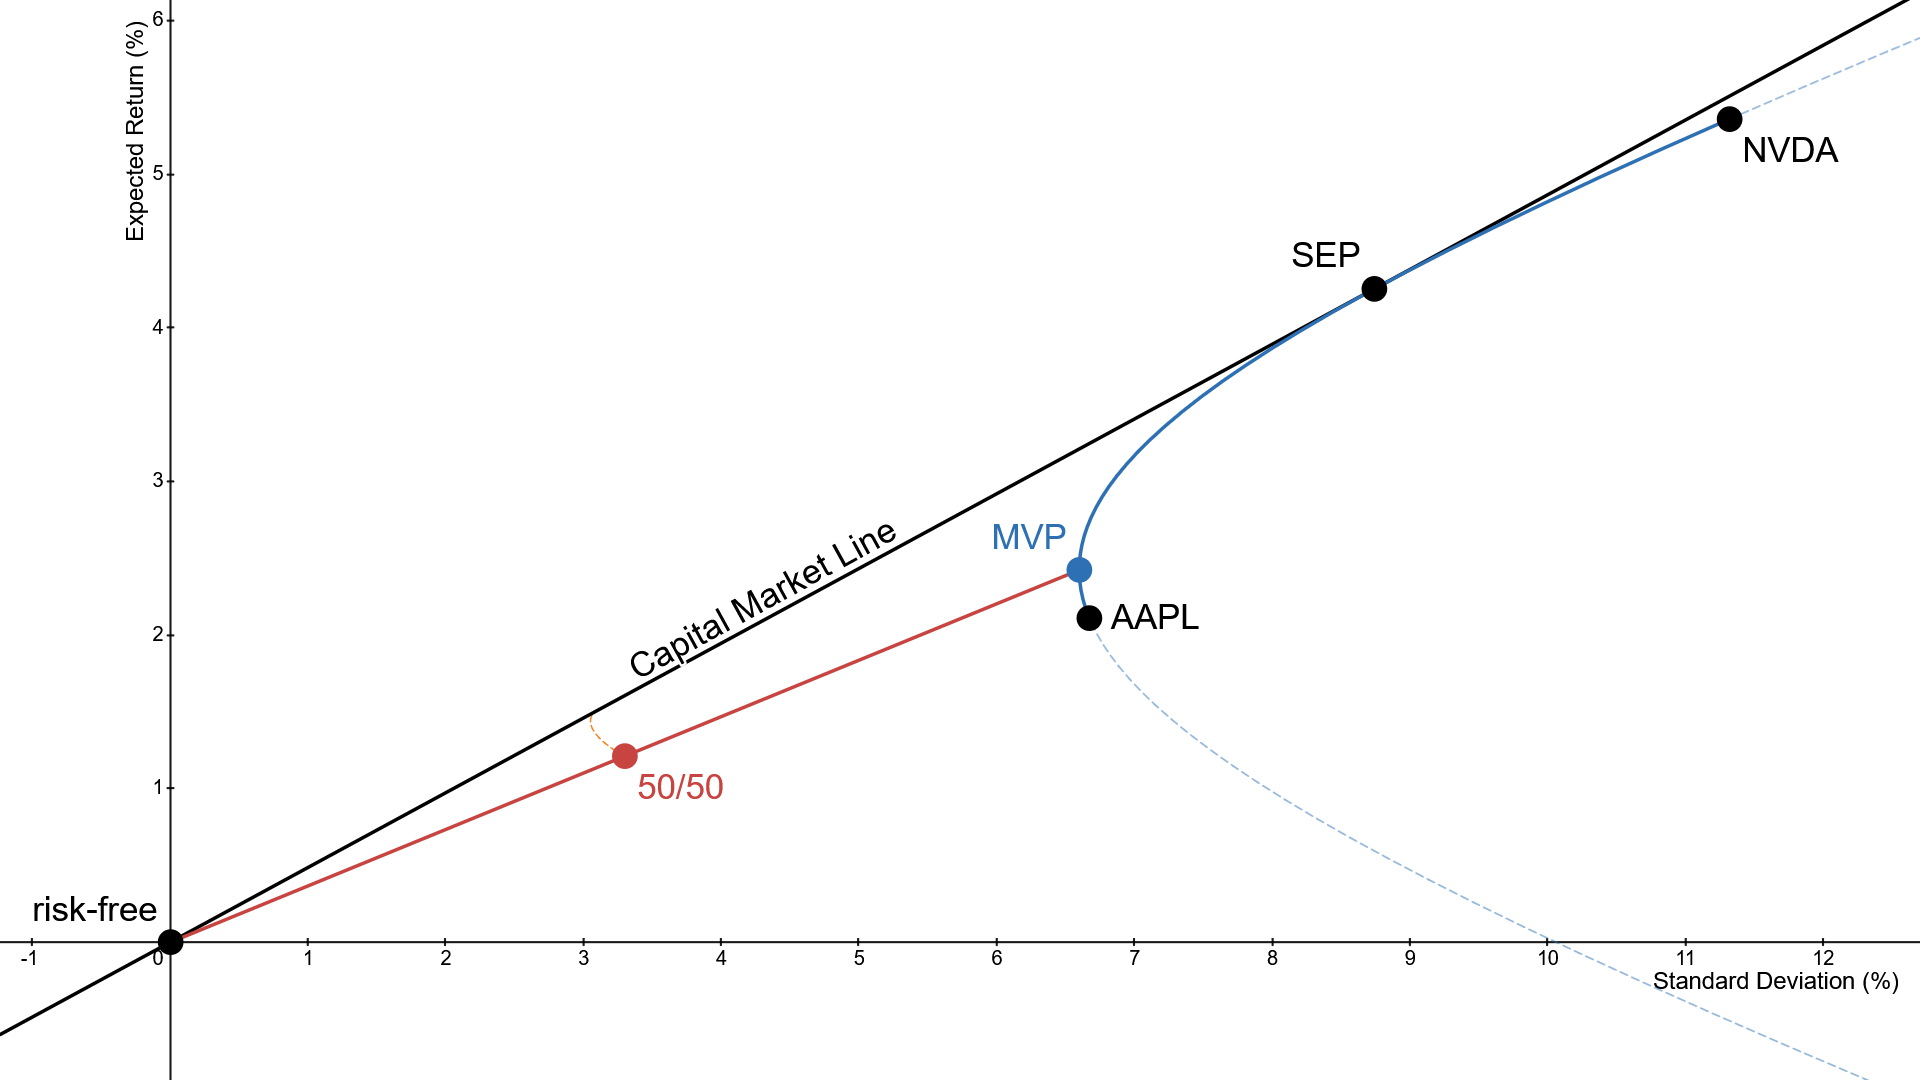
\includegraphics[width=0.25\textwidth]{images/portfolio-analysis.png}
\end{center}